\documentclass[12pt,a4paper,onecolumn]{article}
\usepackage[utf8]{inputenc}
\usepackage{amsmath}
\usepackage{amsfonts}
\usepackage{amssymb}
\usepackage{graphicx}
\usepackage[left=1.50cm, right=1.50cm, top=0.00cm, bottom=0.00cm]{geometry}
\author{Alan}
\title{Primeiro texto Minicurso de Latex}
\begin{document}

\tableofcontents
\newpage



\begin{center}
\textbf{\large Banco de Dados}\vspace{1.5cm}
\end{center}
\begin{abstract}
		Este artigo tem como propósito apresentar as definições de Banco de Dados, incluindo suas diferenças, semelhanças, vantagens e desvantagens
\end{abstract}

\section{O que é Banco de Dados?}

\section{O que são SGBD's?}

	\textbf{SGBD} - É conhecido como sistema gerenciador de banco de dados, ela cuida
	de todo o tratamento de concorrências e recuperação de erros do banco de dados.
	
\begin{figure}[!h]
	\centering
	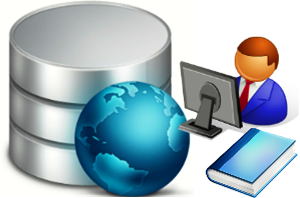
\includegraphics{bd.png}
	\label{figura}
	\caption{banco de dados}
\end{figure}
	
\section{Tipos de Banco de Dados}	

\begin{itemize}
	\item\textbf{Relacional:} O que o torna relacional é a maneira como os dados são armazenados e organizados no banco de dados. Quando falamos em banco de dados, aqui, nos referimos a um banco de dados relacional — RDBMS Relational Database Management System. Em um banco de dados relacional, todos os dados são guardados em tabelas.
	\item\textbf{Não Relacional:}

	
\begin{itemize}
		\item[a.] Orientado a Documento: os documentos dos bancos dessa categoria, são coleções de atributos e valores, onde um atributo pode ser multi-valorado.
		
		Em geral, os bancos de dados orientados a documento não possuem esquema, ou seja, os documentos armazenados não precisam possuir estrutura em comum.
		
		Essa característica faz deles boas opções para o armazenamento de dados semi estruturados.
		\item[b.] Orienado a Grafo: diferentemente de outros tipos de bancos de dados NoSQL, esse está diretamente relacionado a um modelo de dados estabelecido, o modelo de grafos. A ideia desse modelo é representar os dados e/ou o esquema dos dados como grafos dirigidos, ou como estruturas que generalizem a noção de grafos .
		
		O modelo de grafos é mais interessante que outros quando “informações sobre a inter-conectividade ou a topologia dos dados são mais importantes, ou tão importante quantos os dados propriamente ditos .
		
		O modelo orientado a grafos possui três componentes básicos: os nós (são os vértices do grafo), os relacionamentos (são as arestas) e as propriedades (ou atributos) dos nós e relacionamentos.
		
		
		\item[c.] Chave Valor: sistemas distribuídos nessa categoria, também conhecidos como tabelas de hash distribuídas, armazenam objetos indexados por chaves, e possibilitam a busca por esses objetos a partir de suas chaves.\\
		
		
		\begin{tabular}{|c|c|c|c|c|}
		\hline SQL & Rápido & Gestão de informação & Flexível & Integridade de Informação \\
		\hline NoSQL & Menos ágil & Alta disponibilidade & Maior escabilidade & Livres de esquema \\
		\hline 
		\end{tabular} 
		
		
		
\end{itemize}	
\end{itemize}	
	
\end{document}